
%!TEX root = ./main.tex
%** 50_integration.tex
\chapter{Extending FACT with Server Sockets\label{chapter:integration}}

%%%%%%%%%%%%%%%%%%%%%%%%%%%%%%%%%%%%%%%%%%%%%%%%%%%%%%%%%%%%%%%%%%%%%%%%%%%%%%%%
% Smart Traffic Selection using Server Sockets Sets
%%%%%%%%%%%%%%%%%%%%%%%%%%%%%%%%%%%%%%%%%%%%%%%%%%%%%%%%%%%%%%%%%%%%%%%%%%%%%%%%
\section{Smart Traffic Selection using Server Sockets Sets\label{section:ses_traffic_selection}}
% explain briefly the approach / adjustments to FACT
Originally, \gls{FACT} applies a port-based heuristic for selecting the 
examination traffic. 
In detail, \gls{FACT} selects in a first step all traffic towards an external 
\gls{TCP} port 80 originated from an internal client high port. 
Generally, this kind of traffic is denoted as the reflector traffic. 
Then, \gls{FACT} examines each connection from the reflector traffic if it is 
balanced or unbalanced, thus creating an initial set of potential events. 

\begin{figure}
	[!b] \centering
	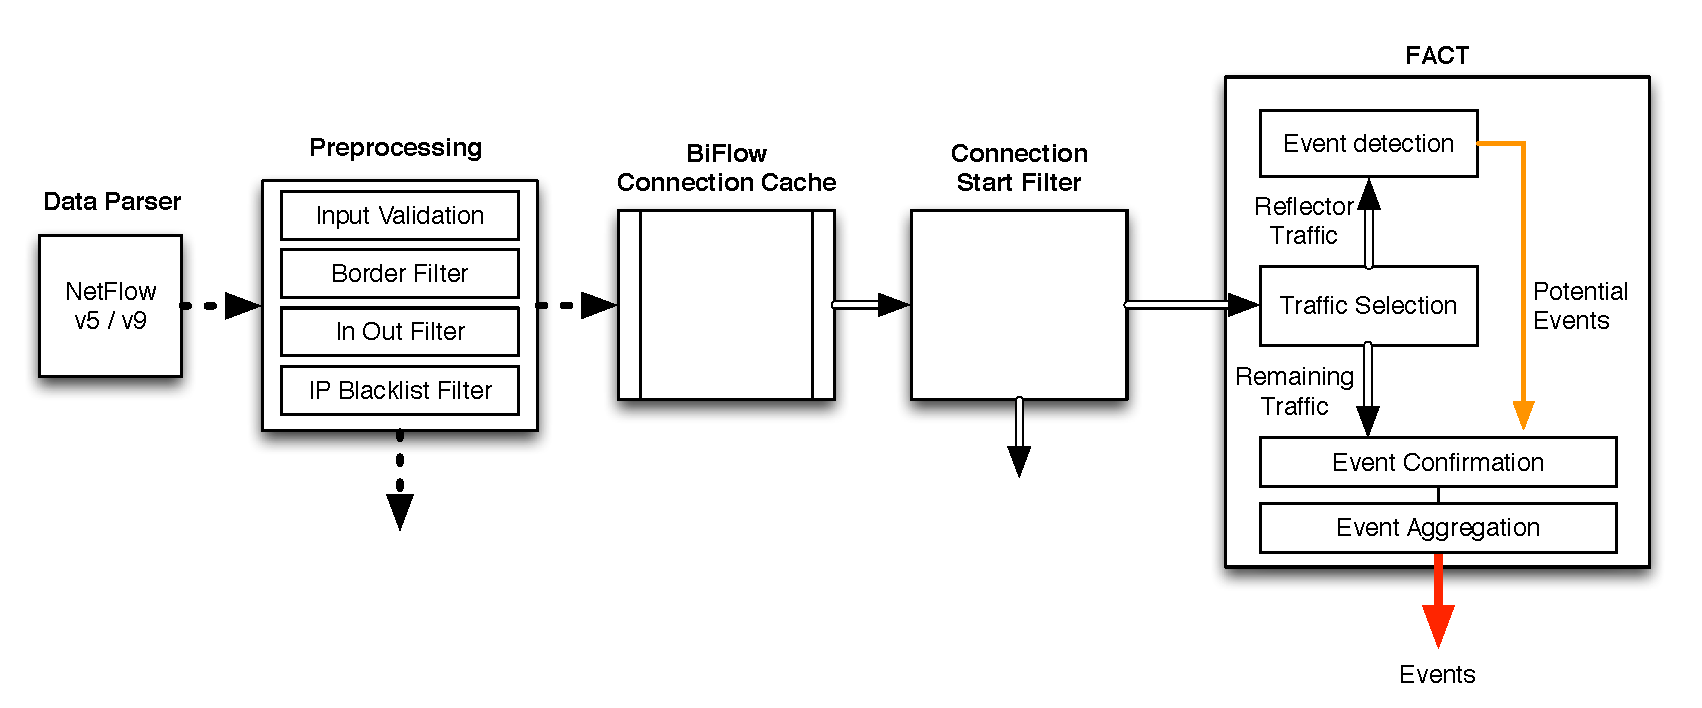
\includegraphics[width=\linewidth]{images/FACT.eps}
	\caption{Processing chain for FACT} 
	\label{fig:fact_chain} 
\end{figure}

In a second step, all potential events inferred by the reflector traffic are 
double-checked with the remaining traffic if a potential event is indeed a 
event. Only if there are no successful connections at all, i.e. all connections 
are unbalanced, a host, network or prefix is declared as unreachable. Otherwise, 
if there is other traffic towards these hosts, networks, and prefixes with 
balanced connections, the potential event is obviously not confirmed and thus 
removed from the event list. 

Since the \gls{server socket} approach aims to replace the port-based heuristic, 
only the generation of the reflector traffic set must be adjusted. The further 
processing steps remain exactly the same. Figure \ref{fig:fact_chain} 
illustrates the \gls{FACT} processing chain and makes clear that only the block 
of the traffic selection must be adjusted to examine traffic towards 
\glspl{server socket} as reflector traffic. This is achieved by loading the 
\gls{server socket} registry with a set of \glspl{server socket}. Then, the 
adjusted traffic selection is querying the server socket registry if the 
external socket is a known \gls{server socket}. If this is the case, the flow is 
added to the reflector traffic, otherwise to the remaining traffic. 

\section{Optimal Server Sockets Sets\label{section:ses_selection}}
% outline that this is a optimization problem which is approximated by several 
% socket sets however not guaranteed to be optimal
% coverage network space / problem space 
By adjusting the traffic selection of \gls{FACT} with \gls{server socket} sets, some essential properties of \gls{FACT} as the observed network coverage or the event sensibility are directly dependent on properties of the chosen 
\gls{server socket} set. 

Because \gls{FACT} detects only network outage events which are firstly detected with the reflector traffic and then not whitelisted by the remaining traffic, it is able to detect only network outages of prefixes which have at least one known 
server socket that is located in this prefix. This means that FACTs observation 
coverage of networks is completely defined by the network/prefix coverage of the 
chosen \gls{server socket} set. 

Obviously, it makes no sense to select for example the 10 most popular sockets 
if they are all located in the same network and prefix, because this set would 
just achieve a network coverage of 1 network/prefix. Hence, the network coverage 
can be optimized by selecting the best socket of these 10 and then select 9 
different sockets which are all located in different networks/prefixes. By doing 
so, the network coverage can be increased. However, if a selected 
\gls{server socket} is not contacted during an observation period the 
observation coverage of this network is lost, unless there is another contacted 
socket located in this network. 
This shows that the selection of \glspl{server socket} is cumbersome and 
directly influences the observation capabilities of FACT. It also shows the 
importance of the visibility and popularity characteristics of \glspl{server socket} 
with respect to the selection in a \gls{server socket} set. 

A popular \gls{server socket} which is always contacted by at least one client 
is able to cover the entire network, because even if this socket is not 
reachable during an observation period the network is further investigated by 
the remaining traffic. 
This is because the unbalanced connection of this \gls{server socket} 
will trigger a potential event which is then confirmed or whitelisted by the 
remaining traffic towards this network. Otherwise, if a socket is not popular 
and only rarely visible, it will not generate a potential event, and hence, the 
event is not detected at all, even if there is a lot of unbalanced traffic 
towards this network contained in the remaining traffic. 

Therefore, the selection of the \glspl{server socket} is basically an optimization 
problem. The goal is to select those sockets with good stability, popularity and 
visibility characteristic without loosing to much network coverage. This problem 
can even be harder if the number of sockets is limited, then the socket density 
of each network must be considered, so that only the few best sockets located in 
a single network are selected. It can even make sense to include not perfectly 
stable sockets if they increase the network coverage, especially if they have a 
good visibility / popularity.

